\chapter{Introduction}
\label{the-introduction}
% This should cover the problem the thesis addresses, the aims and questions, the thesis structure, a summary of the main findings and a discussion on the thesis' contribution. It should prime the reader for what's about to come by providing an overview of what lies ahead.

% Establish your research territory by situating your research in a broader context. 
% Establish and justify your niche by describing why your research is needed. 
% Explain the significance of your research by describing how you conducted your research.
Billions of people use mobile apps on two main mobile platforms Google Android and Apple iOS and their related operating systems, and Android is integrated into additional mobile platforms including Kindle OS and various Chinese manufacturer's devices. There are millions of these mobile apps developed by millions of developers across the globe. Failures in these apps can adversely affect the experiences of end-users, businesses who provide apps, and/or goods and services through mobile apps. 

This thesis focuses on the most used operating system - Android - in it's most popular and mature platform - Google Android - to discover whether mobile analytics can help the developers improve the stability of their apps. A default mobile analytics service is integrated into the Google Android platform and available free of charge for all developers of apps in the Google Play App store so it was selected as the default analytics tool for this research as it is prevalent, widespread, and also one of the quality signals Google uses to decide whether to promote apps in their app store. The default mobile analytics service is complemented with research in additional analytics tools to provide perspective and contrast in their various characteristics and capabilities.

\yijun{Should talk about quality (echoing the title), then talk about reliability and other quality issues.}

As Febrero, Moraga and Calero note~\emph{``Software Quality is a multidimensional concept for which Reliability is considered as a key attribute."}~\citep{febrero2017_software_reliability_as_user_perception}.

Broadly, the research is to understand whether mobile analytics can help developers to improve the reliability of their apps. A second applied research area emerged as various flaws and limitations were discovered in the various mobile analytics services, to discover and categorise the flaws and limitations, and to consider some of the effects of these flaws and limitations. 

In the research developers were able to improve the measured reliability for each of the case studies despite the flaws and limitations. Some improvements were gained with small amounts of effort, others were performed through more strategic changes including replacing Java code with Kotlin replacements and retiring buggy modules and external libraries.  

\begin{comment}
    \begin{itemize}
        \item Get the audience to identify with someone or something, - Give that someone or something some kind of need, - And start changing the circumstances.
        \item Have that someone or something deal with the new circumstances - And find the thing that was needed.
        \item Have that someone or something pay the price of the find - And start heading back toward the original circumstances.
        \item show how those original circumstances have changed as a result.
    \end{itemize}
    \emph{Dan Harmon's story telling circle}
\end{comment}

Before going into details, I will introduce the basis for my theoretical perspective in terms of the ontology and epistemology.

\section{Ontology and Epistemology}
\begin{itemize}
    \item Ontology \( \rightarrow \) a theory of `being' (existence).
    \item Epistemology \( \rightarrow \) what we can know about the microcosm/the world and how we can know it (a theory of knowledge).
\end{itemize}

Both these terms are taken from~\cite{marsh2002skin}. While the article is aimed at social science research, it introduces both topics and their relationships clearly and practically~\footnote{Note: newer versions of the introductory material is published in a book: \href{https://www.macmillanihe.com/page/detail/Theory-and-Methods-in-Political-Science/?K=9781137603517}{\emph{``Theory and Methods in Political Science (\nth{4} Edition)".}}}.

\subsection{Ontology}
Analytics exist and are used across and throughout software development practices. Software is not perfect, it's formed through numerous human endeavours using flawed tools and techniques, no practical software is bug-free, however those involved can improve software through their choices and practices.

[Almost] anything can be measured sufficiently to be useful. In (\cite{hubbard2014measure}) \emph{How to measure anything, \nth{3} edition} the author argues that anything can be measured and proposes an approach to do so. His framework, called \emph{Applied Information Economics: A Universal Approach to Measurement} is summarised in five steps:

\begin{enumerate}
    \item Define the decision.
    \item Determine what you know now.
    \item Compute the value of additional information. (If none, go to step 5.)
    \item Measure where the information value is high. (Return to steps 2 and 3 until further measurement is not needed.)
    \item Make a decision and act on it. (Return to step 1 and repeat as each action creates new decisions.)
\end{enumerate} %~\cite{hubbard2014measure} (page 9).

This approach helps to frame this research into applying analytics to development practices, especially in terms of the practical aspects and nature of real-world apps, development teams, and user-bases..

\subsection{Epistemology}
Here we consider the questions: (1a) What we can know about mobile analytics and (1b) how we can know it? Then more specifically, these related questions are key given this research focuses on using mobile analytics to help answer the next question. (2) How we know about the identification and measurement of some flaws in behaviour of software that are considered measures of quality of the software in use? Broadly we can learn from people, use software tools, and use data to answer these questions. In some cases the data comes from a single source, in others cases from several.

\textbf{Toolbox of methods, how can we know about mobile analytics and the effects of using them?} 

Mobile analytics comprises software, systems, and sometimes services. Broadly we can read about them, study their source code, analyse, test, and use them directly, and ask others for their perspectives and insights. Rather than go into lots of detail here, several of the appendices of this thesis cover aspects of mobile analytics, in particular, in~\href{chapter-on-mobile-analytics}{\emph{\nameref{appendix-on-mobile-analytics}}}. 

In terms of learning from people, we can do so by asking the designers, constructors, operators, and users of a system. However, we're also limited by who we can ask, what they are willing/able to communicate, and whether that communication is sufficiently open and transparent to be useful and reliable. We can also learn from information produced by people, and in particular for mobile apps we can use ratings and reviews. Given human behaviour it may also be worth considering aspects such as the provenance of the information sources, fake data, \emph{etc.} especially where there are rewards for slewing the results of the measurements being used in an ecosystem. 

We can know through static analysis tools, automated tests, end-to-end testing, \emph{etc.} and all of these are used by at least some of the developers of mobile apps some of the time. They often take place \textit{before} the software is released to end users.

We can also know through data collected when the software is used. As~\cite{RFC3164} notes in RFC3164, ~\emph{``Since the beginning... operating systems, processes and applications were written to send messages of their own status, or messages to indicate that certain events had occurred. These event messages generally had local significance to the machine operators."}. Mobile apps also write messages locally and developers use them for similar purposes (nuances and differences are discussed in the related work chapter). These local messages can be read by humans locally and/or read by software that delivers them elsewhere. Developers can also add software to their apps to log information for processing elsewhere which is where much of mobile analytics and crash reporting fits in the scheme of things.

Log messages are written locally on the same device (\textit{i.e.} computer) that runs the software. When developers are developing the software they tend to be local to the device and therefore able to read the logs. When the devices are remote, as they are for end users of mobile apps, developers cannot easily access the logs or read them. If they wish to do so they need mechanisms to obtain the logs. They can choose to incorporate mechanisms into the app including custom logging mechanisms that transmit the logs so they can be processed remotely. They can rely on log forwarding software~\footnote{For instance a fairly involved example for Flutter Android apps, using MQTT, is described in~\citep{adil2020_sending_logs_from_flutter_apps}}, and/or mechanisms provided on the device if they exist. 
% A couple of Android implementations for LogStash include:
%  https://github.com/Labgoo/android-logstash-logger
%  https://gist.github.com/PatrykGala/55603fe4259d812fdc0ffbc9e63eaabc (saved in my references)


Various data can be potentially collected implicitly and explicitly. What can be collected depends on the observation mechanisms. Observation may be within an app or external to it, for instance by the operating system as both iOS  and Google Android do~\footnote{There are other custom versions of Android, for instance used in Amazon Kindle Fire devices. Their details are outside the scope of my research.}(details in the Appendix titled~\href{chapter-on-mobile-analytics}{\emph{\nameref{appendix-on-mobile-analytics}}}). Within an app the observation may focus at a single layer, for instance the visual user interface, or several. The choices of observation mechanisms within an app are made by developers or their stakeholders. The choices external to an app can be made by various people including the platform provider, users, or indirectly using other software including third-party apps, spyware, accessibility software, and so on.

Analytics, such as user-journeys, can help to answer questions about the usage of the software. They help establish \emph{what-is}. As we understand more about what-is we can then consider \emph{what-would-be-better} and do gap analysis between what-is and what-would-be-better.

Reporting/generating and Observing... What happens within the app stays within the app unless someone looks inside the app or the app reports what's occurring. Observation without action limits the utility of whatever is learned. 

Survivorship bias (\cite{wikipedia_survivorship_bias}) is relevant to understanding the information developers receive, some data does not `survive' the journey from source to developer. And much of the information that is does reach the developers does not survive or, perhaps better put, thrive in terms of being used productively. They have plenty of other demands for their time and attention and much of what could be useful isn't used in practice, therefore the data needs to be sufficiently useful and relevant and improvements tractable for any proposed approach to be used long term in practice.



\section{The Research}
Software app developers need to deliver software that can be used successfully by end users. To do so they need to be able to create software and distribute it so it is available to end users. They need to do so in a timely manner, and perfection may be too long to wait for. End users need to be able to install and use that software. If the software is sufficiently usable, useful and behaves adequately they may continue to use it. Developers cannot assess \emph{a priori} whether their software will meet the needs and expectations of users, meet their needs, or the needs of their stakeholders. In short they do not know whether it will thrive.

One of the key considerations is whether the quality of their apps are adequate. There are many ways to assess quality of apps, including static analysis, in-person testing, and automated testing. Users may perform their own subjective assessments of quality and some of these users provide feedback in the form of ratings and reviews. 

Researchers have investigated these various sources of quality related information. My research concentrates on using sources of analytics related to usage of apps to help developers a) assess the quality of their current software, and b) improve the quality using the same analytics sources.

This research was inspired by learning about the power and capabilities of applying usage data collected by mobile apps in extremely popular real-world mobile apps in the early days of mobile apps (before Android, iOS and other modern mobile platforms were released). At the time I worked for Google and was responsible for testing all Google's mobile apps, including: Search, GMail, Maps, and many others.

Several years later, when consulting with another company with over ten million active users I discovered they had included two analytics tools in their apps where there were numerous discrepancies in the data collected, the ways the counted and the resulting reports, yet they were both considered necessary. The engineers then added a third analytics library in the hope it would correlate with one or other of the existing libraries - it didn't, instead it had distinct characteristics and counts. And yet the developers were able to discover how their apps were used in incredible detail and by applying what they learned their apps became increasingly popular and financially successful.

These experiences led me to starting my PhD in order to research the potential of mobile analytics, and to understand some of their flaws and the effects of those flaws. During my research there have been incredible changes in the mobile landscape (for instance major manufacturers, operating systems, etc. have appeared, mushroomed, and disappeared). Similarly many test automation tools and frameworks have been and gone. Meanwhile, apps and app stores have spread beyond smartphones and tablets to desktop operating systems, cloud-based product offerings such as Salesforce, etc. Google's Android platform includes platform-level data collection, reporting and analytics intended to help developers learn about ways they can improve their apps. Meanwhile regulation has started to emphasise and highlight some of the many risks and concerns with gathering data wantonly. 

Despite all these changes, and my limited inroads into a subset of the entire landscape, the research seems to indicate the potential of applying usage analytics to improve both the product (the software) and the process (how the software is developed and tested). The research also identified flaws within analytics tools and also between analytics tools. Both the potential and the flaws appear worth sharing with researchers and with practitioners to help them chose and use analytics wisely.


\subsection{Research Problem}
Research into the use and efficacy of software usage analytics appears to be under-served, particularly in terms of being able to use the analytics to identify and potentially address quality flaws in apps in use. And in recent years, platform-wide analytics has been made available to all the developers of actively used Android apps in Google Play. Despite the ubiquity of these platform-level analytics there appeared to be no research into their efficacy, completeness, or accuracy.


\subsection{Research Contributions}
The research presents the results of several case studies in the use of analytics to improve the reliability of a variety of mobile apps.

TBC. Answer: ``how your work contributes to the field" (see \url{https://uofgpgrblog.com/pgrblog/the-viva-exam}), and your ``contribution to knowledge"~\url{https://www.theguardian.com/higher-education-network/2015/jan/08/how-to-survive-a-phd-viva-17-top-tips}

\subsection{Research Scope}
Developers have various sources of feedback about their apps, as Figure~\ref{fig:sources-of-feedback-for-developers} illustrates. The pink triangle represents the extent of Google Play (the app store) in terms of providing feedback. Other feedback is also available independently of the app store, for instance by using software incorporated directly into the app and from the development process.

\begin{figure}[htbp!]
    \centering
    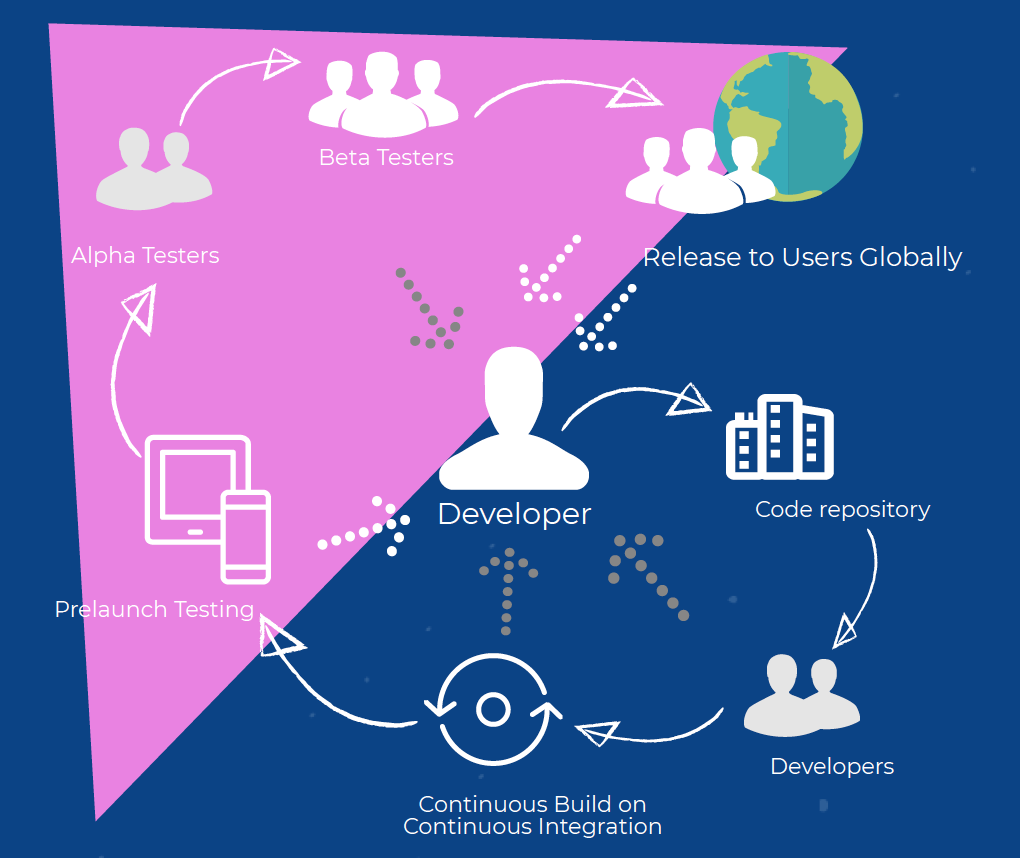
\includegraphics[width=13cm]{images/silvias-developer-centric-figure-mobilesoft2020.png}
    \caption{Sources of feedback for developers}
    \label{fig:sources-of-feedback-for-developers}
\end{figure}

Each source of feedback may stem from humans (for example, in reviews) or from software (for example, from code quality tools such as Lint). This research introduces three sources of software generated feedback.

\subsection{Research Strategy}


\section{Findings}\label{findings-section}
\yijun{Is it too early to reveal the findings here? Maybe you can prepare the reviewers by presenting the findings as confirmation of some "hypothesis", and first discuss about these hypothesis before introducing the facts? It will be good to move 1.5 Research Questions here and articulate them as hypothesis or early hypothesis?}

The application of mobile analytics has enabled each of the development teams who participated in the research to materially improve their measured reliability. 

For the first case study the reliability was improved approximately 12x for the main Kiwix Android application by applying the approach identified in this research. 
During the initial improvement stages the reliability of the project's custom apps did not improve. These custom apps are built using the main application's source code, and when the improved codebase was used to create new releases of the custom apps their reliability also improved several fold.

\begin{figure}[htbp!]
    \centering
    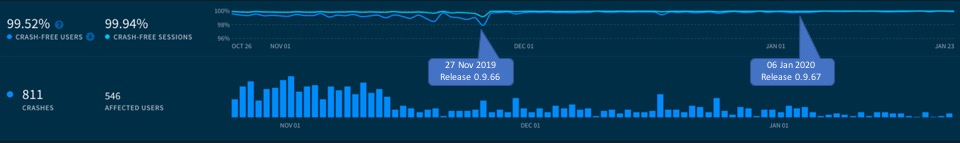
\includegraphics[width=\textwidth]{images/annotated_pocketcode_90_day_fabric_crashlytics_report.jpg}
    \caption{Pocket Code improvements in crash rate, in 90 days}
    %\Description{Pocket Code: When the project team investigated crashes they improved the reliability}
    \label{fig:pocketcode_improvements_in_crash_rate}
\end{figure}

An unacceptably high crash rate for the key Pocket Code Android app were tamed within two releases and 7 weeks by applying the approach described in this thesis. The changes needed to make the improvements were small. Figure \ref{fig:pocketcode_improvements_in_crash_rate} shows the improvement in crash rate as measured by Fabric Crashlytics. When the experiment started the crash rate was nearly four times the maximum threshold recommended by Google in their Android Vitals service and the project team had not been able to address the crash rate despite applying many of the recognised and recommended software development practices over several years~\cite{adamsen2015systematic_catrobat, luhana2018streamlining, ali2019behavior_catrobat, ali2019using_catrobat, hirsch2019approach_catrobat, schranz2019contributors_catrobat, slany2014tinkering}.

The developers continue to actively use mobile analytics to highlight potential quality issues and address pertinent issues promptly. One of the project teams chose to add an additional analytics tool to both their Android and iOS apps with the objective of improving the teams understanding of broader quality concerns. These quality concerns now also include usability. The team aims to use the data to improve the usability and user experience for their current and future users. They are designing the analytics to retain and protect user privacy, both important and highly relevant concerns.

Mobile Analytics can be incorporated as additional sources of information for development teams in harmony with other sources of information - it is not exclusive or exhaustive.

The analytics tools Google provides to developers of Android apps in Google Play Console have value despite the many flaws my research uncovered in their tools and reports. Some are mentioned in published papers~\cite{harty_google_play_console_insightful_development_using_android_vitals_and_pre_launch_reports, harty_better_android_apps_using_android_vitals, harty_improving_app_quality_despite_flawed_mobile_analytics}, the current known set are in this thesis. The research identified major differences in the reports and analytics provided by two analytics tools from the same company. There were both internal and cross-tool flaws and inconsistencies. Some of these have already been reported to Google in preparation for a full report to be submitted on completion of some ongoing research.

Fully automated pre-launch reports are effective at finding some quality flaws in Android apps at no financial cost and minimal effort by the app developers. These reports are provided by the app store and intended to help developers identify quality issues with their Android apps in order to address these issues so they do not affect end-users.

\subsection{The following section to be revised and moved}

 

Google Play uses data collected automatically from users opted-in to provide usage and diagnostics data to Google. The data is collected at a per-device level, which means that one device could potentially report data from several user accounts, conversely for users who use multiple devices some may provide the data while others do not.


I instigated and led the development of several opensource software utilities to help record and preserve reports and underlying failure data from Google Play Console and Android Vitals. We have successfully extended the capabilities of the utilities and further extensions are practical. Research benefits:
\begin{itemize}
    \item Evidence preserved for analysis:
    \item Data can now be compared and further assessed:
    \item Data and contents can be shared by developers of Android apps with other researchers - extending the body of knowledge about crashes (un-reliability) and ANRs (run-time unresponsiveness). \emph{bringing previously unknown data, practices and tools into the open so others can understand them, make more informed decisions, and perform further research.}
\end{itemize}

I made data available~\cite{harty_wama_dataset_examples} for further research based on data originally only made available to app developers. Larger volumes of data are available upon request.

The research has been presented at various conferences and workshops, including at NII Shonan~\footnote{NII Shonan hosts highly collaborative workshops on various topics with participants from multiple continents~\citep{acm_shonan_workshops_2020}.} in 2019 at meeting 152 on "Release Engineering for Mobile Applications"~\footnote{~\url{https://shonan.nii.ac.jp/seminars/152/}}. 

\section{Outline of this thesis}
Bugs are ubiquitous in software (even one of the most respected software engineers, Donald E. Knuth, recognises, publicly acknowledges, \emph{and pays for}~\cite{knuth_trutex, wikipedia__knuth_reward_checks_2020} bugs found in his creations. And self-aware developers expect there will be bugs in their software. \emph{``You are entitled to a reward of at least 0x$1.00 ($2.56) if you are the first person to report a bona-fide error not on those lists."} Donald E. Knuth~\cite{knuth_the_bank_of_san_serriffe}

Even top development teams are likely to learn of bugs they were not able to find, and cannot reproduce. For instance, Google's Android Auto Team have asked for help from end users to identify patterns that may help the team find and address a long-running and frustrating bug in Android Auto~\footnote{\url{https://support.google.com/androidauto/thread/2865341?msgid=44437416}}. As reported by \texttt{autoevolution} in May 2020:  
\emph{"As it turns out, the Android Auto team wasn’t able to reproduce the whole thing, so it’s now asking users to send additional reports with more information to help fix the problem."}~\footnote{~\url{https://www.autoevolution.com/news/google-wants-users-to-help-fix-widespread-android-auto-bug-143760.html}}.


\subsection{Validation of the concepts}
My practical research focuses on two sets of Android applications, those of the Kiwix and Catrobat project teams. According to data and reports Google provides the development teams their active user-bases are 362,595 for the Kiwix project across 18 published apps, and 148,966 for the Catrobat project across 6 published apps. %data obtained on 16th May 2020.
TODO map these apps to the buckets in the table from the 'beyond Google Play' paper.

While these apps include a useful variety of user populations (from 10's of users to 150K+ across many countries and tens of apps) they could be perceived as a \emph{drop in the ocean} of the millions of apps currently available in the Google Play app store. Also, both project teams are non commercial, and may have different working dynamics from commercial development projects and teams. As my research was inspired from my consulting work with businesses who rely on the success of their apps I chose to supplement these two projects by engaging with developers from several commercial development teams. These include: Moonpig, Moodspace, and LocalHalo. Each values and uses analytics data during their development process to assess post-launch issues with their apps. From time to time things go awry with the behaviours of one or more of their releases and analytics helps them to identify and respond to issues before they become pervasive. For the LocalHalo app, \emph{TODO add details}... For Moonpig \emph{TODO add details}...

\subsubsection{Validation by the Google Engineering Team}
In Spring 2019 I reported various flaws or potential anomalies in various reports Google Play Console provides to developers to the then Product Manager for Android Vitals, Mr Fergus Hurley. As the long-term product owner he has extensive and insider experience of the tools and reports Google provides to an estimated population of over 1 million Android developers \emph{TODO add references e.g. to the Beyond Google Play paper and the one about a few developers creating an exponential number of apps}. I asked for his perspective during both a long in-person meeting and a follow-up video call a few weeks later. He confirmed several of the issues and debated others. He was willing to go on record in one of my accepted peer-reviewed papers on the topic \emph{TODO add link} and asked me to continue to share my findings with them. During the next 12 months he and then they added more Google staff to the discussion and asked me to write up my findings in a document that became over 30 pages long. Their policy means they are unlikely to confirm changes they make as a result of my research and findings, nonetheless they accept and value the feedback that has been provided. They also confirmed various bugs were ones they want to address.
